\section{Detectors}\label{sec:detectors}

In this section we introduce the detector noise curves used in \ref{app:a}. We begin with a description of the basic operation of detectors. We then discuss ground-based detectors, space-based detectors and PTAs in turn. The latter function somewhat differently than conventional interferometers, so we include a brief introduction to PTA analysis. References for the noise curves used for individual detectors can be found in the relevant subsections and further information about the detectors can be discovered in these. Detectors are frequently upgraded and redesigned, hence, while these curves are believed to be correct at the time of writing, it is best to check for updates from the appropriate science teams before relying on the details given here, although we hope that they shall remain accurate enough for illustrative purposes.

\subsection{Operating principle of an interferometric detector}\label{sec:principles}

All of the man-made detectors discussed in this section utilise the principle of interferometry. Such detectors work by taking a beam of monochromatic light and splitting it into two beams travelling at some angle to each other. Each beam is passed in to an optical cavity where it undergoes a number of round trips before being recombined to form an interference pattern. The ends of the cavity are, in the ideal case, freely floating test masses which move in response to a passing GW, this effect is measured by observing the changing interference pattern.

The response of a detector to an incident plane-fronted GW depends upon the relative orientations of the detector and the incoming wave. Let us choose the origin of our coordinate system to be the beam-splitter of the interferometer, and $l_{1}^{i}$ and $l_{2}^{i}$ to be unit 3-vectors pointing along the two arms. In the absence of noise the output of the detector is the difference in strain between the two arms \citep{Thorne1987}
\begin{equation}\label{eq:hoftxx}
h(t)=\frac{1}{2}h_{ij}\left( l_{1}^{i}l_{1}^{j}-l_{2}^{i}l_{2}^{j} \right)\; ,
\end{equation}
where $h_{ij}$ are the spatial components of the GW metric perturbation. Let $\hat{r}^{i}$ be the unit 3-vector pointing towards the source of the GWs, with spherical polar angles $(\theta,\phi)$ relative to some axes fixed to the detector, and let $p^{i}$ and $q^{i}$ be unit vectors orthogonal to $\hat{r}^{i}$. We can now define the basis tensors
\begin{eqnarray}
H^{+}_{ij}&=p_{i}p_{j}-q_{i}q_{j} \; , \\
H^{\times}_{ij}&=p_{i}q_{j}+q_{i}p_{j} \; .
\end{eqnarray}
There remains a freedom in the coordinates described, a rotation of $p^{i}$ and $q^{i}$ through an angle $\psi$ about $\hat{r}^{i}$ known as the polarization angle. For a single frequency component, the strain induced by a GW may be written as
\begin{equation}\label{eq:hijxx}
h_{ij}=A_{+}H^{+}_{ij}\cos\left(2\pi ft\right)+A_{\times}H^{\times}_{ij}\cos\left(2\pi ft+\Delta \phi\right) \; ,
\end{equation}
where $A_{+}$ and $A_{\times}$ are the amplitudes of the two polarisation states. Combining (\ref{eq:hoftxx}) and (\ref{eq:hijxx}) allows the detector output to be written as
\begin{equation}
h(t)=F^{+}(\theta,\phi,\psi)A_{+}\cos\left(2\pi ft\right)+F^{\times}(\theta,\phi,\psi)A_{\times}\cos\left(2\pi f t + \Delta\phi \right)\; ,
\end{equation}
where the response functions inherit their angular dependence from the choice of coordinates
\begin{eqnarray}\label{eq:responsefuncs}
F^{+}(\theta,\phi,\psi)&=\frac{1}{2}H^{+}_{ij}\left(l_{1}^{i}l_{1}^{j}-l_{2}^{i}l_{2}^{j}\right) \; , \\
F^{\times}(\theta,\phi,\psi)&=\frac{1}{2}H^{\times}_{ij}\left(l_{1}^{i}l_{1}^{j}-l_{2}^{i}l_{2}^{j}\right) \; . 
\end{eqnarray}

The response function of a two-arm interferometric detector is quadrupolar, an example is plotted in figure \ref{fig:LIGO}.
\begin{figure}
 \centering
 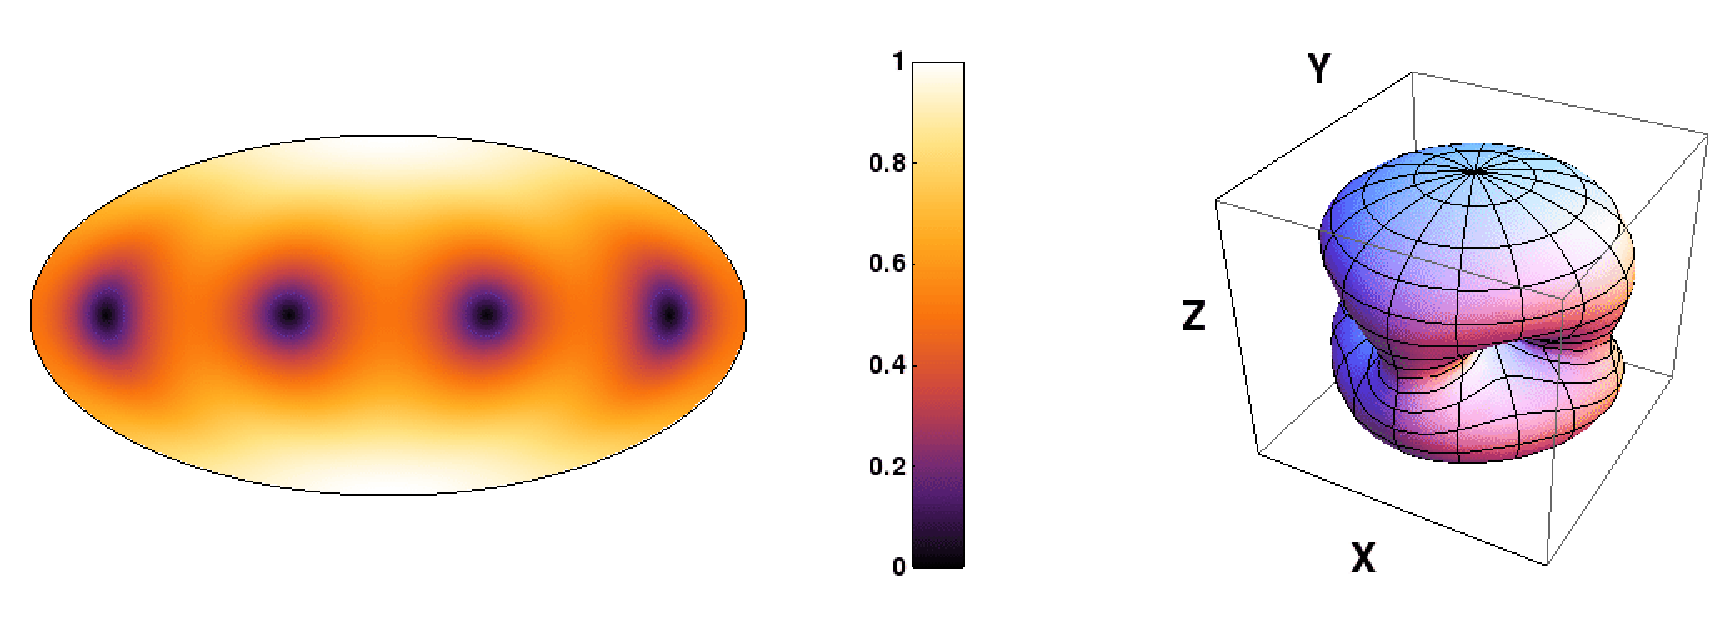
\includegraphics[trim=0cm 0cm 0cm 0cm, width=0.99\textwidth]{LIGO_detectorframe.pdf}
 \caption{The angular response function of an interferometric detector shown both as a surface plot and in an Aitoff--Hammer projection. The quantity that is plotted is is the polarisation average, $\left[(1/2\pi)\int\mathrm{d}\psi \;(F^{+})^{2}+(F^{\times})^{2}\right]^{1/2}$. The response is a function of two sky angles, $\theta$ and $\phi$, and varies between $0$ and $1$. The two detector arms lie in the $x$--$y$ plane either side of one of the zeros in the response.}
 \label{fig:LIGO}
\end{figure}
Throughout this paper detector sensitivity refers to the polarisation and sky averaged sensitivity $F$, where
\begin{equation}\label{eq:skyav}
F^{2}=\int_{0}^{2\pi}\frac{\mathrm{d}\psi}{2\pi}\; \int_{0}^{2\pi} \frac{\mathrm{d}\phi}{2\pi}\; \int_{0}^{\pi}\frac{\sin\theta\,\mathrm{d}\theta}{2}\;\left[F^{+}\left(\theta,\phi,\psi\right)^{2}+F^{\times}\left(\theta,\phi,\psi\right)^{2}\right]\; .
\end{equation}
For a single $90\degree$-interferometer, such as LIGO, the sky and polarisation averaged response is $F=\sqrt{1/5}\approx 0.447$.

A detector may consist of several interferometers. Let $F_{a}$ be the averaged response of the $a$-th interferometer, the average response of a network of $k$ detectors is obtained by adding in quadrature,
\begin{equation} F_{\mathrm{Total}}^{2}=\frac{1}{k}\sum_{a\,=\,1}^{k}F_{a}^{2} \; .\end{equation}

The averaging in (\ref{eq:skyav}) assumes a uniform distribution of polarisation angles $\psi$. This is the case for a stochastic background; however, for a non-inspiralling circular binary, the polarisation is a function of the two spherical polar angles ($\iota,\xi$) specifying the orientation of the binary's orbital angular momentum. Here, $\iota$ is the inclination angle, the polar angle between the orbital angular momentum and the line joining the source to the detector ($-\hat{r}$) and $\xi$ is the azimuthal angle around the same line. In this case, to characterise the detector sensitivity we average over all four angles ($\theta,\phi,\iota,\xi$). If the binary is inspiralling, then the polarisation depends on still more parameters which need to be averaged over. These more complicated averages all have the property that they depend on both the detector and the source, hence they are unhelpful for our present purpose separating the source amplitude from the detector sensitivity. Additionally, the different averages do not work out to be so different from each other: \citet{1993PhRvD..47.2198F} calculated the sensitivity for a detector with the LIGO geometry averaged over the four angles ($\theta,\phi,\iota,\xi$) as $\sqrt{4/25}=0.4$ times peak sensitivity, which should be compared with the value $\sqrt{1/5}\approx 0.447$ above. The effect of replacing the true sensitivity with the sky-averaged sensitivity for the LISA detector was considered in detail by \cite{2012CQGra..29l4015V}; they also found there is a small difference when considering an entire population of sources. For the remainder of this paper the three-angle average defined in (\ref{eq:skyav}) is used.

\subsection{Ground-based detectors}\label{sec:ground}

Ground-based detectors are the most numerous. A collection of interferometric detectors are listed in table \ref{table:t}, these are sensitive to GWs in the frequency range ${\mathcal{O}}(10$--$10^{3})~\mathrm{Hz}$. They all simulate free-floating test masses by suspending a mass from a pendulum system with natural frequency much greater than that of the GW. Their sensitivity curves include narrow lines that arise from noise sources in the instrument, including resonances in the suspension system and electrical noise at multiples of $60~\mathrm{Hz}$: these have been removed in the \ref{app:a} figures for clarity. The detectors fall broadly into three categories: first-generation detectors, which have already operated; second-generation detectors currently under construction; and third-generation detectors at the planning stage. 

The most notable ground-based detectors are LIGO and Virgo, which work in collaboration, supported by GEO600. LIGO, Virgo and GEO600 have completed science runs as first-generation detectors \citep[e.g.,][]{Abadie2010}. As LIGO and Virgo are currently being upgraded their initial configurations are now referred to as Initial LIGO (iLIGO) and Initial Virgo (iVirgo) respectively. The upgraded, second-generation versions are referred to as Advanced LIGO (aLIGO) and Advanced Virgo (AdV) respectively. LIGO has two observatories: one at Hanford, Washington, which has two detectors; and another at Livingston, Louisiana. There is an agreement to move one of the upgraded Hanford detector systems to a location in India \citep{LIGO-India,Unnikrishnan2013}. The GEO600 detector is not subject to a major upgrade plan, but since summer 2009 it has enhanced by a series of smaller improvements, notably improving high-frequency sensitivity \citep[GEO-HF;][]{2006CQGra..23S.207W}. The advanced detectors should start operation in the next couple of years, with LIGO-India following further in the future.

TAMA300 is a Japanese first-generation detector. Its successor, currently under construction, is the Kamioka Gravitational Wave Detector (KAGRA), formerly the Large-scale Cryogenic Gravitational wave Telescope (LCGT), which is located underground in the Kamioka mine. It employs more sophisticated noise-reduction techniques than LIGO or Virgo, such as cryogenic cooling.

The Einstein Telescope (ET) is an ambitious proposal to construct an underground third-generation detector. Its location would provide shielding from seismic noise, allowing it to observe frequencies of $10$--$10^4~\mathrm{Hz}$. 

\begin{table}
\caption{\label{table:t} Summary of ground-based laser interferometers.}
\begin{indented}
\item[]\begin{tabular}{ l l l l l }
\br
{\bf Detector} & {\bf Country} & {\bf Arm length} & {\bf  Approximate date} & {\bf Generation} \\
\mr
  GEO600$^{a}$	&	Germany 	& $600~\mathrm{m}$ 	& 2001--present	   & First \\
  TAMA300$^{b}$ & 	Japan		& $300~\mathrm{m}$ 	& 1995--present    & First \\
  iLIGO$^{c}$	&	USA		& $4~\mathrm{km}$ 	& 2004--2010 	   & First \\
  Virgo$^{d}$	& 	Italy		& $3~\mathrm{km}$ 	& 2007--2010 	   & First \\
  aLIGO$^{e}$	&	USA		& $4~\mathrm{km}$ 	& \emph{est.} 2015 & Second \\
  AdV$^{f}$	&	Italy	 	& $3~\mathrm{km}$ 	& \emph{est.} 2016 & Second \\
  KAGRA$^{g}$	&	Japan		& $3~\mathrm{km}$ 	& \emph{est.} 2018 & Second \\
  ET$^{h}$      & 	---		& $10~\mathrm{km}$ 	& \emph{est.} 2025 & Third \\
\br
\multicolumn{5}{l}{$^{a}$\citet{2010CQGra..27h4003G}, $^{b}$\citet{2002CQGra..19.1409A}, $^{c}$\citet{2009RPPh...72g6901A},}\\
\multicolumn{5}{l}{$^{d}$\citet{accadia_virgo:2012}, $^{e}$\citet{2010CQGra..27h4006H}, $^{f}$\citet{Acernese2009}, $^{g}$\citet{2012CQGra..29l4007S}, $^{h}$\citet{2011CQGra..28i4013H}.}\\
\br
\end{tabular}
\end{indented}
\end{table}

We use an interpolation to the data published on \url{https://wwwcascina.virgo.infn.it/advirgo/} (2013) for the AdV sensitivity curve, an interpolation to the data for version D of the KAGRA detector published on \url{http://gwcenter.icrr.u-tokyo.ac.jp/en/researcher/parameter} (2013) and analytic fits to the sensitivity curves from \citet{Sathyaprakash} for the remaining detectors.

\subsection{Space-based detectors}\label{sec:space}

Space-based detectors work on similar principles to ground based detectors, but with the test masses residing inside of independent, widely separated satellites. Space-based detectors are sensitive to lower frequency GWs than their ground-based counterparts; this is partly because space-based detectors can have much longer arms, and partly because they are unaffected by seismic noise which limits the low frequency performance of ground-based detectors. 

The canonical design for a space-based detector is the Laser Interferometer Space Antenna (LISA), which is sensitive to millihertz GWs. LISA would consist of three satellites flying in a triangular constellation with arms of length $5\times 10^{9}~\mathrm{m}$ in a $1~\mathrm{AU}$ orbit around the Sun, trailing the Earth by $20\degree$. The laser arms in a LISA-like detector are not a cavity, the light only travels once along each arm. eLISA is a rescoped version of LISA designed to probe the same frequency range, while proposals such as the Advanced Laser Interferometer Antenna (ALIA), Big Bang Observer (BBO) and Deci-hertz Interferometer GW Observatory (DECIGO) are designed to probe decihertz GWs.

\subsubsection{LISA and eLISA}

The instrumental noise curves for LISA are approximated by the analytic fit given by \citet{Sathyaprakash}, which we use for the plots in \ref{app:a}. When observing individual sources with LISA there is an additional contribution to the noise from a background of unresolvable binaries. This is not included here as we consider the background as a source of GWs (see section \ref{sec:GB}). eLISA is a rescoped version of the classic LISA mission, the main differences are shorter arms ($10^{9}~\mathrm{m}$ instead of $5\times 10^{9}~\mathrm{m}$), two laser arms instead of three, and a different orbit (drifting away from Earth instead of $20\degree$ Earth trailing). The effect of these changes is a slightly reduced peak sensitivity and a shift to higher frequencies. We use an analytic fit to the instrumental noise curve given by \citet{Amaro-Seoane-et-al}.

\subsubsection{DECIGO, ALIA and BBO}

These missions are designed to probe the decihertz region of the GW spectrum; they are considerably more ambitious than the LISA or eLISA mission and their launches will be further into the future. We use a simple analytic fit to the sensitivity curve for ALIA~\citep{bender_possible_2013}, while for DECIGO and BBO, fits to the sensitivity curves given by \citet{2011PhRvD..83d4011Y} are used.

\subsection{Pulsar timing arrays}\label{sec:PTAgeneralproperties}

PTAs can be thought of as naturally occurring interferometers with galactic-scale arm lengths. Accordingly, they are sensitive to much lower frequencies than the detectors previously discussed. Each pulsar is a regular clock and the measured pulse arrival time can be compared against a prediction, leaving a residual which includes the effects of passing GWs. Using an array of these pulsars spread across the sky allows us to correlate residuals between different pulsars, to exploit the fact that GWs influence all pulsars whereas intrinsic pulsar noise does not. The correlation between different pulsars depends only on their angular separation on the sky, and has a distinctive shape, known as the Hellings and Downs curve \citep{HellingsDowns}.

The redshift of the rate of arrival of pulses for a pulsar at a distance $L$ from the Solar-System barycentre (SSB), in the direction of the unit spatial vector $\hat{p}$ induced by a GW travelling in direction of the unit vector $\hat{\Omega}$ is \citep{anholm-2009}
\begin{equation}\label{eq:pulsarredshift}
z(t,\hat{\Omega})= \frac{1}{2} \frac{\hat{p}^{j}\hat{p}^{i}} {1+\hat{\Omega}\cdot\hat{p}}\left[h_{ij}^{\mathrm{Pulsar}}\left(t-\frac{L}{c},\hat{\Omega} \right)-h_{ij}^{\mathrm{Earth}}(t,\hat{\Omega} )\right] = \frac{1}{2}\frac{\hat{p}^{j}\hat{p}^{i}}{1+\hat{\Omega}\cdot\hat{p}} \Delta h_{ij}(t,\hat{\Omega})\; .
\end{equation}
The redshift includes two terms: the pulsar term and the Earth term. The pulsar term is often neglected in PTA analysis as it can be considered as an extra noise term which averages to zero across the array. The experimentally measured quantity is not the redshift but the timing residual, the two are related via
\begin{equation}\label{eq:restored}
R(t,\hat{\Omega}) = \int_{0}^{t}\mathrm{d}t'\;z(t',\hat{\Omega}) \; .
\end{equation}
All of the pulsars, and the Earth, are subject to the same metric-perturbation field. This may be expressed in terms of its Fourier transform
\begin{equation}
h_{ij}(t,\vec{r}) = \sum_{A\,=\,+,\,\times}\int\mathrm{d}f\;\iint_{\mathbb{S}_{2}}\mathrm{d}\hat{\Omega}\; \tilde{h}_{A}(f,\hat{\Omega})e_{ij}^{A}(\hat{\Omega}) \exp\left[2\pi i f \left(t-\frac{\hat{\Omega}\cdot\vec{x}}{c}\right)\right] \; ,
\end{equation}
where $e^{A}_{ij}(\hat{\Omega})$ is the $A$ polarisation basis tensor for direction $\hat{\Omega}$  and $\vec{r}$ is the spatial position. Choosing the SSB as the origin of our coordinate system, so the pulsar is at position $L\hat{p}$, gives
\begin{equation}\label{eq:deltahij}
\Delta h_{ij}(t,\hat{\Omega}) = \sum_{A\,=\,+,\,\times}\int\mathrm{d}f\; \tilde{h}_{A}(f,\hat{\Omega})e_{ij}^{A}(\hat{\Omega})\exp\left(2\pi \rmi f t\right)\left\{\exp\left[-2\pi\rmi fL \left(1+\hat{p}\cdot\hat{\Omega}\right)\right]-1\right\} \; .
\end{equation}
From (\ref{eq:pulsarredshift}) and (\ref{eq:deltahij}), the Fourier transform of the redshift $\tilde{z}(f,\hat{\Omega})$ can be identified as
\begin{equation}\label{eq:45}
\tilde{z}(f,\hat{\Omega}) = \left\{\exp\left[-2\pi\rmi fL \left(1+\hat{p}\cdot\hat{\Omega}\right)\right]-1\right\} \sum_{A\,=\,+,\,\times} \tilde{h}_{A}(f,\hat{\Omega})F^{A}(\hat{\Omega}) \; ,
\end{equation}
where
\begin{equation}
F^{A}(\hat{\Omega}) = \frac{e_{ij}^{A}(\hat{\Omega})\hat{p}^{j}\hat{p}^{i}} {2\left(1+\hat{\Omega}\cdot\hat{p}\right)} \, .
\end{equation}
The function $F^{A}(\hat{\Omega})$ may be regarded as the PTA equivalent of the detector response functions in (\ref{eq:responsefuncs}). The stochastic background of GWs is fully characterised by the one-sided PSD via the expectation value
\begin{equation}\label{eq:stochback}
\left<\tilde{h}_{A}^{*}(f,\hat{\Omega})\tilde{h}_{A'}(f',\hat{\Omega}')\right> = \frac{1}{2}S_{h}(f)\delta^{(2)}(\hat{\Omega}, \hat{\Omega}')\delta_{AA'}\delta(f-f') \; ,
\end{equation}
where $\delta^{(2)}(\hat{\Omega},\hat{\Omega}')$ is the delta-function on the sphere. From (\ref{eq:45}) and (\ref{eq:stochback}), the expectation of the product of signals from two different pulsars in directions $\hat{p}_{1}$ and $\hat{p}_{2}$ may be evaluated as
\begin{equation} 
\left<\tilde{z}_{1}(f)\tilde{z}_{2}^{*}(f')\right> = \frac{1}{2}S_{h}(f)\delta (f-f')\Gamma(f) \; ,
\end{equation}
where
\begin{eqnarray}
\Gamma(f) &= \sum_{A\,=\,+,\,\times} & \iint_{{\mathbb{S}}^{2}}\mathrm{d}\hat{\Omega}\,\left\{\exp\left[2\pi\rmi fL_{1}\left(1+\hat{\Omega}\cdot\hat{p}_{1}\right)\right]-1\right\} \nonumber \\*
 & & \times \left\{\exp\left[-2\pi\rmi fL_{2}\left(1+\hat{\Omega}\cdot\hat{p}_{2}\right)\right]-1\right\} F_{1}^{A}(\hat{\Omega})F_{2}^{A}(\hat{\Omega}) \; .
\end{eqnarray}
The overlap function $\Gamma(f)$ tends to a constant value in the limit that the distances to the pulsars are large compared to the wavelength of GWs; PTAs operate in this limit, so the overlap may be approximated as a constant, 
\begin{equation}
\Gamma(f) \approx \Gamma_{0} = \sum_{A\,=\,+,\,\times}\iint_{{\mathbb{S}}^{2}}\mathrm{d}\hat{\Omega}\;F_{1}^{A}(\hat{\Omega})F_{2}^{A}(\hat{\Omega})\;.
\end{equation}
Neglecting the exponential terms in the overlap is the frequency-domain equivalent of neglecting the pulsar term in (\ref{eq:pulsarredshift}). The integral may be evaluated to give an expression depending only on the angle $\theta$ between the two pulsars; this is the famous Hellings and Downs curve, shown in figure \ref{fig:HnD},
\begin{equation}
\Gamma_{0} = \frac{1}{2}+\frac{3\xi}{2}\left(\ln \xi -\frac{1}{6}\right) \; ,
\end{equation}
where $\xi = (1-\cos\theta)/{2}.$
\begin{figure}
 \centering
 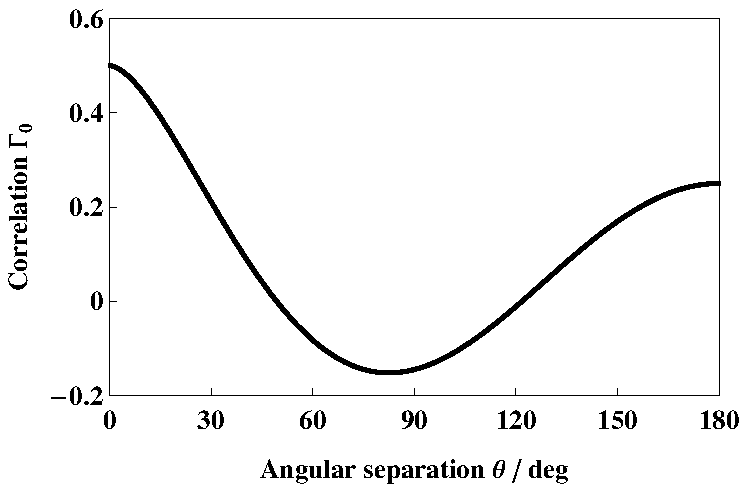
\includegraphics[trim=0cm 0cm 0cm 0cm, width=0.55\textwidth]{Fig_Hellings_Downs}
 \caption{The \citet{HellingsDowns} curve, the correlation between two pulsars separated on the sky by an angle $\theta$.}
 \label{fig:HnD}
\end{figure}

The sensitivity bandwidth of a PTA is set by the sampling properties of the data set. If measurements are spaced in time by $\delta t$ and taken for a total length of time $T$, then the PTA is sensitive to frequencies in the range $(1/T) < f < (1/\delta t)$. The characteristic strain that the PTA is sensitive to scales linearly with $f$ in this range. This gives the wedge-shaped curves plotted in \ref{app:a}. The absolute value of the sensitivity is fixed by normalising to a calculated limit at a given frequency for each PTA. For a discussion of the sensitivities of PTA to both individual sources and stochastic background, see \citet{MooreTaylorGair}.

There is a discrepancy between the treatment of PTA sensitivity curves here and the higher frequency detectors discussed in sections \ref{sec:ground} and \ref{sec:space}. When observing a long-lived source, such as an inspiral, with a high frequency detector the convention was to define a \emph{characteristic} strain to satisfy (\ref{eq:hc}). Here, the convention is to leave the strain untouched and instead adjust the PTA sensitivity curve with observation time, again to satisfy (\ref{eq:hc}). This discrepancy is an unfortunate result of the conventions in use by the different GW communities; however, it is natural given the sources under observation. When observing a transient source, such as a burst or inspiral, which changes within the lifetime of the detector, it is natural to consider the detector as performing constantly while the signal changes. However, when observing a monochromatic source or a stochastic background, which is unchanging over the detector lifetime, it is more natural to consider the source as being fixed and the sensitivity of the detector gradually improving. All that is required by the definition in (\ref{eq:hc}) is that the ratio $h_\mathrm{c}(f)/h_{n}(f)$ is constant.


\subsubsection{Current PTAs}

The PTAs currently in operation are the European Pulsar Timing Array \citep[EPTA\footnote{\url{http://www.epta.eu.org/}};][]{eptareview2013}, the Parkes Pulsar Timing Array \citep[PPTA\footnote{\url{http://www.atnf.csiro.au/research/pulsar/ppta/}};][]{parkesreview2013} based in Australia, and the North American Nanohertz Observatory for Gravitational waves \citep[NANOGrav\footnote{\url{http://nanograv.org/}};][]{nanogravreview2013}. There are published limits on the amplitude of the stochastic background from all three detectors: the most recent from EPTA is \citet{Haasteren}, from PPTA is \citet{Shannon2013} and from NANOGrav is \citet{2013ApJ...762...94D}. The limits from the existing detectors are all of a similar magnitude; the PPTA limit is a factor of $\sim 2.5$ lower than the other two. In \ref{app:a} we use the EPTA limits, this was based on an analysis of $5$ pulsars over approximately $10~\mathrm{yr}$. The curve labelled ``EPTA'' is normalised to agree with the limit published in \cite{Haasteren} at a frequency of $f_{0}=1~\mathrm{yr^{-1}}$.

\subsubsection{The International Pulsar Timing Array}

Combining the existing arrays would yield a single PTA using approximately $4$ times as many pulsars; this consortium of consortia is known as the International Pulsar Timing Array \citep[IPTA\footnote{\url{http://www.ipta4gw.org/}};][]{iptareview2013}. The IPTA curves plotted in the figures are based on $20$ pulsars timed for twice as long as the current EPTA.

\subsubsection{SKA}

The next great advancement in radio astronomy shall come with the completion of the Square Kilometre Array \citep[SKA;][]{Dewdney2009}. This shall greatly increase the sensitivity of pulsar timing \citep{Kramer2004}. The sensitivity curves plotted in \ref{app:a} for the SKA assume a root-mean-square error on the timing residuals a factor of $10$ better than current PTAs, and include $20$ pulsars timed for twice as long as the current EPTA.

